\documentclass{beamer}

\usepackage[utf8]{inputenc}
\usepackage{default}
\usepackage{graphicx}

% TODO Learn what this does
% source
% http://tex.stackexchange.com/questions/15952/layout-of-multiple-lines-footnotes
% this is a way to adjust foot note so it can be cutted into multiple lines
\makeatletter
\renewcommand\@makefntext[1]{\tiny\rightskip=25em\hskip0em\@makefnmark#1}
\makeatother

\makeatletter
\newcommand*{\rom}[1]{\expandafter\@slowromancap\romannumeral #1@}
\makeatother


% shows how to change default (blue) colours in the default beamer theme
% found here: http://joerglenhard.wordpress.com/tag/latex/
\definecolor{WaterlooRed}{RGB}{145,11,46}
\setbeamercolor{title}{fg=WaterlooRed}
\setbeamercolor{frametitle}{fg=WaterlooRed}
\setbeamercolor{structure}{fg=WaterlooRed}

% adds logo in the footer
\logo{
\includegraphics[scale=.25]{img/csuow}}

\title[]{Shoshin Presentation April 2014}
\author[Xu Cui]{Xu Cui}
\institute{
\includegraphics[scale=0.25]{img/UniversityOfWaterloo_logo_vert_rgb.png}}
\date{{\tiny\today}}

\begin{document}

\begin{frame}
  \titlepage
\end{frame}


\begin{frame}
  \frametitle{Agenda}
  \begin{itemize}
  \item Previous Project Report
  \item Future Work
    \begin{itemize}
    \item Motivation
    \item Current Research Topics
    \item Problems Statement
    \item Sketched Approach
    \end{itemize}
  \item Summary
  \end{itemize}
\end{frame}


\begin{frame}
  \frametitle{Previous Project Report}
  \begin{itemize}
  \item MicroFuge is near its completion.
  \item Spent this term polishing the paper.
  \item The paper is accepted to ICDCS. Special thanks to Akshay, Ben, Bernard
    and Khuzaima.\footnote{Ordered by alphabet}
  \item I shall present the paper in Madrid at the beginning of July, 2014.
  \item Most details of MicroFuge were presented in the previous Shoshin
    Meeting and I would like to talk about the work I may work on next.
  \end{itemize}
\end{frame}



\begin{frame}
  \frametitle{Future Work}

  \emph{I need your suggestions and help, feel free to speak up if you have
    anything to say. Anything is fine.

I am interested in all of your ideas.

Just speak up.  Thanks!

}
\end {frame}


\begin{frame}
  \frametitle{Future Work - Motivation}
  \begin{figure}
    \centering
    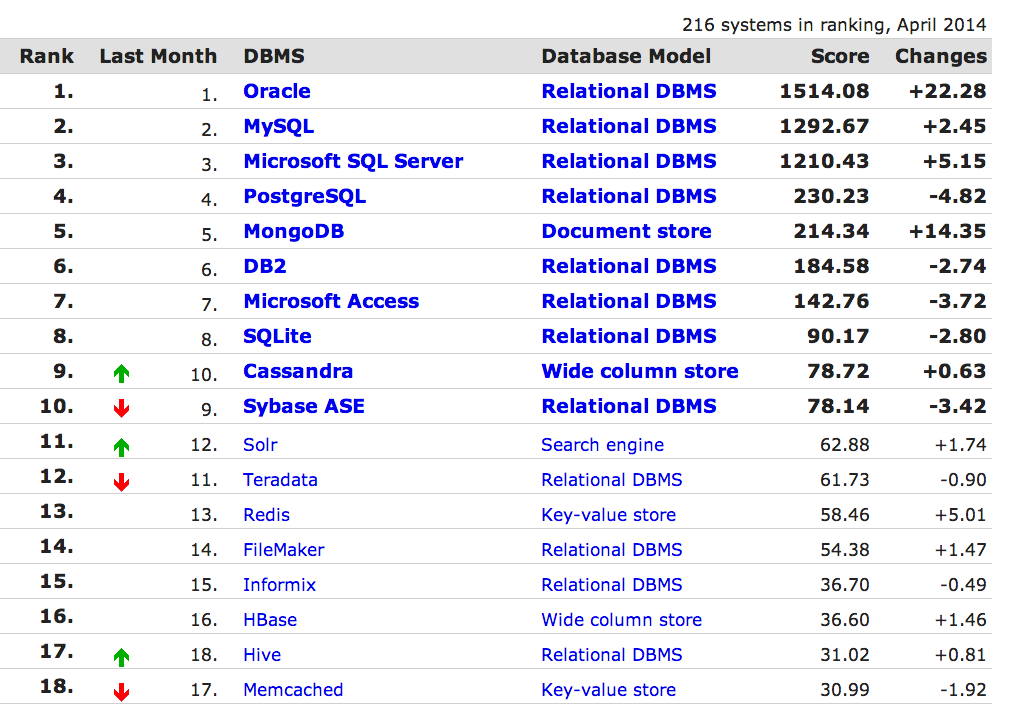
\includegraphics[scale=0.28]{img/DB_Ranking_2014_April.png}
    \caption{Screenshot of DB Ranking from \url{http://db-engines.com}}
  \end{figure}
\end {frame}



\begin{frame}
  \frametitle{Future Work - Motivation}
  \begin{itemize}
  \item The ranking is computed based a variety of information including number
    of mentions on system websites, general interests based on Google trend,
    job offers, etc.
  \item NoSQL databases are gaining its popularity in today's cloud
    environments.
  \item NoSQL data storage provides native horizontal scaling.
  \item NoSQL data storage *provides* better performance.
  \item NoSQL data model addresses large volumes of structured,
    semi-structured or unstructured data.\footnote{According to
      \url{http://www.mongodb.com/}}
  \item etc.
  \end{itemize}
\end{frame}


\begin{frame}
  \frametitle{Future Work - Motivation}
  \begin{itemize}
  \item Query planner is one of the most important cornerstone of a RDBMS.
  \item Traditionally, a query planner is not needed for most NoSQL databases
    because there are not many tuneable knobs to be considered in the query
    planning besides indices.
  \item NoSQL databases are starting to have more tuneable knobs
    \begin{itemize}
    \item e.g. Write Concern of MongoDB, a way to specify write consistency
      levels.\footnote{http://docs.mongodb.org/}
    \end{itemize}
  \item If we can have more optimization options, query planning should be a
    part of the NoSQL databases.
  \end{itemize}
\end {frame}

\begin{frame}
  \frametitle{Future Work - Current Research Topics}
  \begin{itemize}
  \item Some query optimization/planner works are done on NoSQL databases in
    order to combine the use of NoSQL and SQL databases in a single storage
    system.
    \begin{itemize}
    \item Data Integration over NoSQL Stores Using Access Path Based Mappings,
      by Olivier Curé, et al., proposed a middleware system which sits on top
      of several NoSQL stores that processes SQL queries using Access Path
      Based Mappings.
    \item Bridging SQL and NoSQL -- A Master's Thesis by John Roijackers at
      Eindhoven University of Technology.
    \end{itemize}
  \item Not much work has been done in NoSQL databases because only the very
    basic optimizations, nowhere as sophisticated as SQL optimization, have
    been done in limited number of NoSQL databases.\footnote{History Repeats
      Itself: Sensible and NonsenSQL Aspects of the NoSQL Hoopla by C. Mohan at
      IBM Almanden Research Center}
  \end{itemize}
\end{frame}

\begin{frame}
  \frametitle{Future Work - Problem Statement}

  Derive an utility function based on relevant cloud system states(such as
  network conditions), datacenter cost metrics(such as energy consumption) and
  SLAs(such as consistency requirement). Design and implement a query planner
  for the existing NoSQL databases such that it maximizes the utility function
  to provide the optimal query plan with respect to any prioritized view of the
  cost models.

\end{frame}

\begin{frame}
  \frametitle{Future Work - Sketched Approach}
  \begin{itemize}
    \item Study the query languages of the NoSQL databases.
    \item Analyze all possible cost metrics.
    \item Derive the Utility function.
    \item Implement the utility function.
    \item Merge the utility function implementation into the query languages.
    \item Evaluate the performance gain by comparing the cost metrics
  \end{itemize}
\end{frame}

\begin{frame}
  \frametitle{Summary}
  \begin{itemize}
    \item An query planner for NoSQL databases.
    \item Only at the planning stage.
    \item Please provide suggestions and criticisms, the more the merrier.
    \item Thank you!

    \item
      \emph{If you are willing to share with me how you look for your research
        ideas, please speak up. Or you can talk to me personally.

        I would really appreciate your help.
        I am open to any suggestions.}
  \end{itemize}
\end{frame}
\end{document}
